\subsection{Model architecture}

\begin{figure}[t]
    \begin{minipage}{0.64\linewidth}
    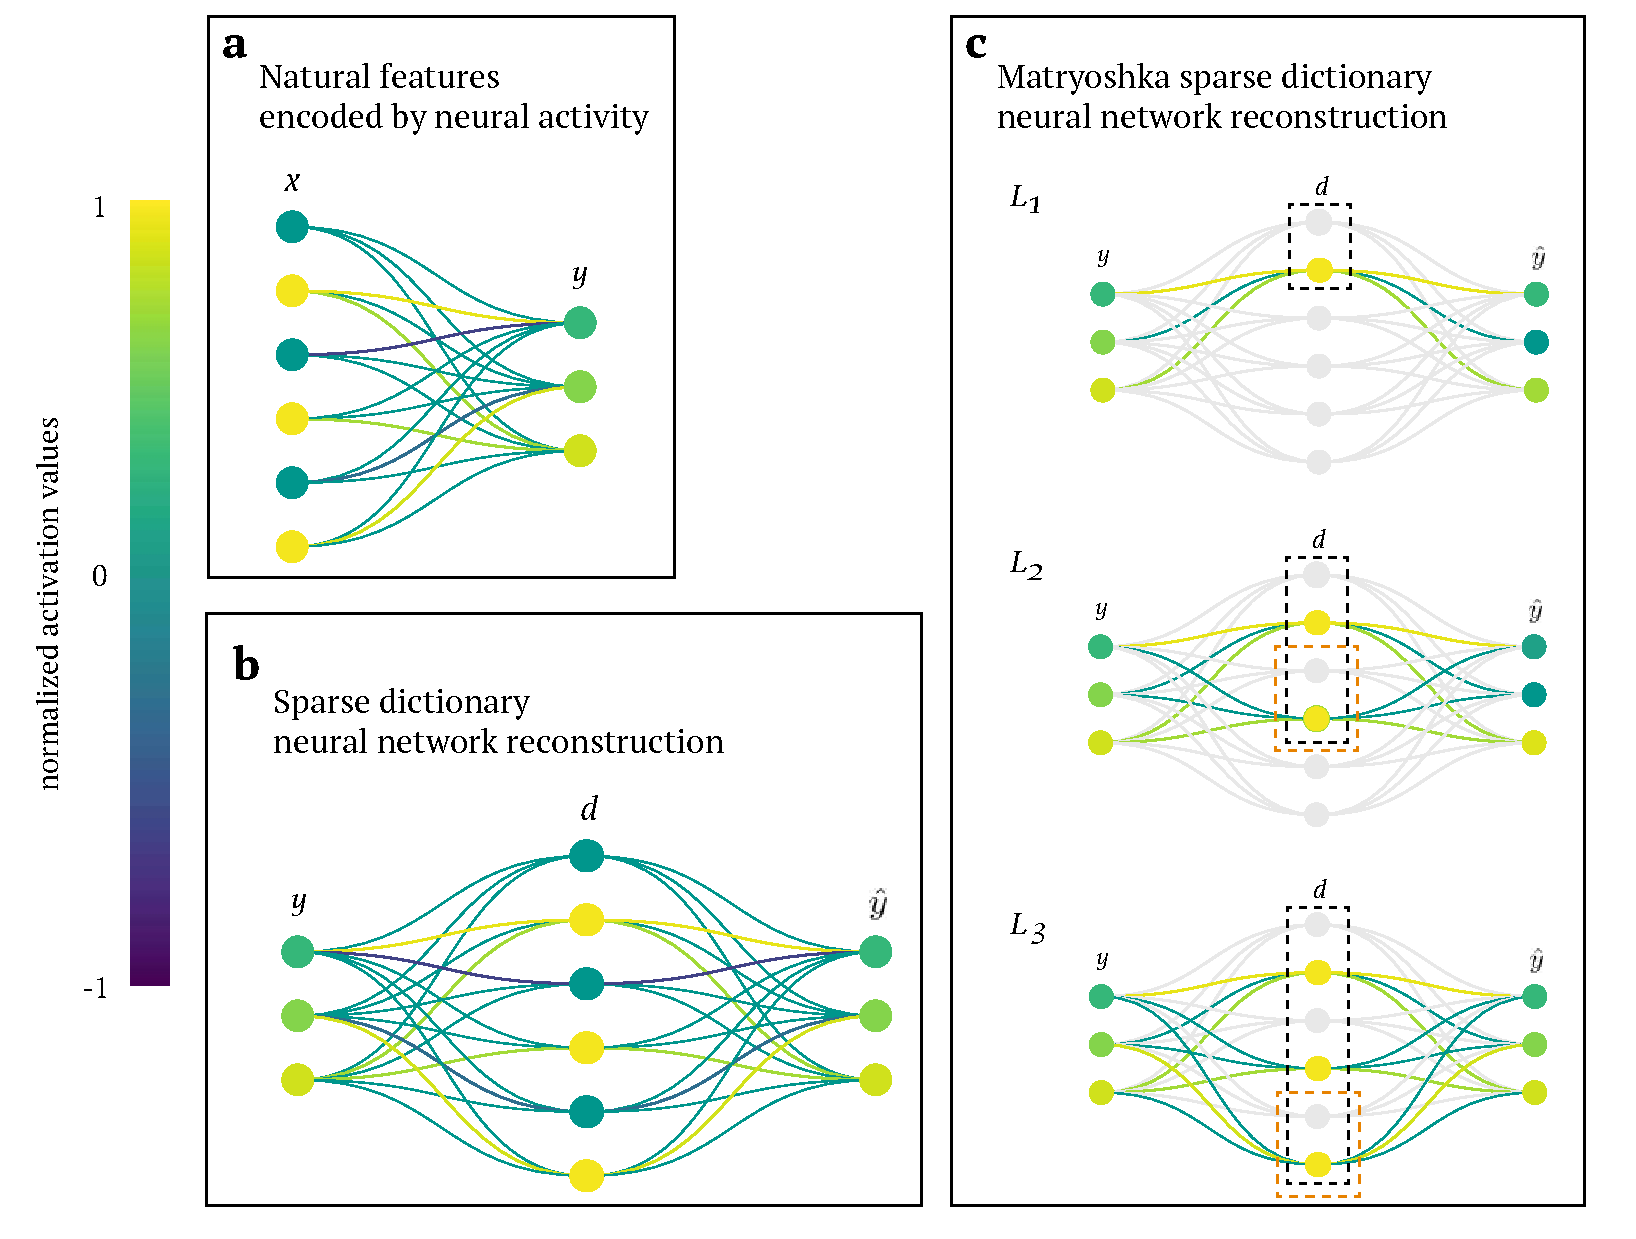
\includegraphics[width=\linewidth]{figures/sdnn_arch.pdf}
    \end{minipage}%
    \begin{minipage}{0.35\linewidth}
    \caption{
        \textbf{Model motivation} \\
        \small
        (\textbf{a}) Natural ("real-world") features $x$ get encoded by neural activity $y$. At this timepoint, three active features are simultaneously represented by the joint activity of three neurons (\textbf{b}). A neural network reconstructs neural activity $\hat{y}$ from $y$ via sparse dictionary elements $d$. When training is successful, $d$ corresponds to $x$: sparse dictionary elements represent natural features. If $\hat{y}$ tries to recreate $y$ exactly, the model is an autoencoder; in other scenarios (e.g. $\hat{y}$ is separate but dependent on or related to $y$) it is a transcoder or crosscoder. ()\textbf{c}) A Matryoshka spare dictionary neural network segments the latent space into multiple levels, each of which attempts to do a full reconstruction of the target neural activity. In this case, latents exclusive to the highest-level will often correspond to high-level features (e.g. a round object), while latents exclusive to the lowest-level will often correspond to low-level features (e.g. a basketball).
    }
    \label{fig:sdnn_arch}
    \end{minipage}
\end{figure}

\begin{itemize}
    \item Usefulness of SDL methods in Mech interp.
    
    \item Variant of MSAE as variant of SAE.
    \begin{itemize}
        \item Briefly mention other archs tried: batchTopK winner for sparsity enforcement.
    \end{itemize}
    
    \item In addition to MSAE levels width, briefly mention hyperparameters, expound in Appendix.
    \begin{itemize}
        \item topk per level, loss X per level, seq len for neural data, seq len for latent space used with transformer layer in decoder
    \end{itemize}
    
    \item Show latex formulas for encoder, decoder, total loss.
\end{itemize}